\documentclass[letterpaper,10pt]{article}
\usepackage[top=2cm, bottom=1.5cm, left=1cm, right=1cm]{geometry}
\usepackage{amsmath, amssymb, amsthm,graphicx}
\usepackage{fancyhdr}
\pagestyle{fancy}

\lhead{\today}
\chead{Quality Engineering Assignment 12}
\rhead{Justin Hood}

\newcommand{\Z}{\mathbb{Z}}
\newcommand{\Q}{\mathbb{Q}}
\newcommand{\R}{\mathbb{R}}
\newcommand{\C}{\mathbb{C}}
\newtheorem{lem}{Lemma}

\begin{document}
\begin{enumerate}
\item We consider the heart attack data. We shall assume normality and control in the data for the purposes of the assignment. First, we compute $\hat{C}_p$ as,
\begin{align*}
\hat{\sigma} &= \frac{\bar{s}}{c_4}\\
&=\frac{1}{0.9693}\\
&=1.03167\\
\hat{C}_p&=\frac{USL-LSL}{6\hat{\sigma}}\\
&=\frac{36-30}{1.03167}\\
&=0.9693\\
&\to 0.97
\end{align*}
Next, we consider $\hat{C}_{pk}$. To compute, we consider the following calculations,
\begin{align*}
\zeta(USL) &= |36-32|\\
&= 4\\
\zeta(LSL) &= |30-32|\\
&=2
\end{align*}
Because we see that the second of these calculations is the smallest, we shall use it in the calculation of our $\hat{C}_{pk}$ value as,
\begin{align*}
\hat{C}_{pk} &= \frac{\bar{\bar{x}}-LSL}{3\hat{\sigma}}\\
&=\frac{32-30}{3(1.03167)}\\
&=\frac{2}{3.09501}\\
&=0.6462\\
&\to 0.65
\end{align*}
Finally, we compute the DPMO as,
\begin{align*}
P(X<LSL) &=\Phi(\frac{30-32}{\hat{\sigma}})\\
&=0.026275032\\
P(X>USL) &= 1-\Phi(\frac{36-32}{\hat{\sigma}}\\
&=0.0000528327\\
P(Defect) &= 0.026275032+0.0000528327\\
&=0.026327865\\
DPMO &= P(Defect)\times 10^6\\
&=26327.86453\\
&\to 26327.9
\end{align*}
\item Next, we consider the Chocolate data. Again, we assume that the process is normally distributed and in control. Then, as before, we compute,
\begin{align*}
\hat{\sigma} &= \frac{\bar{R}}{d_2}\\
&=\frac{2}{2.059}\\
&=0.971345313\\
\hat{C}_p&=\frac{USL-LSL}{6\hat{\sigma}}\\
&=\frac{29-23}{0.971345313}\\
&=1.0295\\
&\to 1.03
\end{align*}
Next, we consider $\hat{C}_{pk}$. To compute, we consider the following calculations,
\begin{align*}
\zeta(USL) &= |29-25|\\
&= 4\\
\zeta(LSL) &= |23-25|\\
&=2
\end{align*}
Because we see that the second of these calculations is the smallest, we shall use it in the calculation of our $\hat{C}_{pk}$ value as,
\begin{align*}
\hat{C}_{pk} &= \frac{\bar{\bar{x}}-LSL}{3\hat{\sigma}}\\
&=\frac{25-23}{3(0.971345313)}\\
&=\frac{2}{2.914035939}\\
&=0.68633\\
&\to 0.69
\end{align*}
Finally, we compute the DPMO as,
\begin{align*}
P(X<LSL) &=\Phi(\frac{23-25}{\hat{\sigma}})\\
&=0.019747119\\
P(X>USL) &= 1-\Phi(\frac{29-25}{\hat{\sigma}}\\
&=0.0000191087\\
P(Defect) &= 0.019747119+0.0000191087\\
&=0.019766228\\
DPMO &= P(Defect)\times 10^6\\
&=19766.22798\\
&\to 19766.2
\end{align*}
\item Next, we consider the strut data. Again, we assume that the process is normally distributed and in control. Then, as before, we compute,
\begin{align*}
\hat{\sigma} &= \frac{\bar{R}}{d_2}\\
&=\frac{1.66}{2.059}\\
&=0.80621661\\
\hat{C}_p&=\frac{USL-LSL}{6\hat{\sigma}}\\
&=\frac{90-70}{6*0.80621661}\\
&=4.134538151\\
&\to 4.14
\end{align*}
Next, we consider $\hat{C}_{pk}$. To compute, we consider the following calculations,
\begin{align*}
\zeta(USL) &= |90-73.58|\\
&= 16.42\\
\zeta(LSL) &= |70-73.58|\\
&=3.58
\end{align*}
Because we see that the second of these calculations is the smallest, we shall use it in the calculation of our $\hat{C}_{pk}$ value as,
\begin{align*}
\hat{C}_{pk} &= \frac{\bar{\bar{x}}-LSL}{3\hat{\sigma}}\\
&=\frac{73.58-70}{3(0.80621661)}\\
&=\frac{3.58}{2.41864983}\\
&=1.480164659\\
&\to 1.48
\end{align*}
Finally, we compute the DPMO as,
\begin{align*}
P(X<LSL) &=\Phi(\frac{70-73.58}{\hat{\sigma}})\\
&=0.00000448763\\
P(X>USL) &= 1-\Phi(\frac{29-25}{\hat{\sigma}}\\
&\approx 0\\
P(Defect) &= 0.00000448763+0\\
&=0.00000448763\\
DPMO &= P(Defect)\times 10^6\\
&=4.48763\\
&\to 4.5
\end{align*}
\item Finally, we consider the air data provided. First, we compute a histogram of the data, and see that it is roughly normal,
\begin{center}
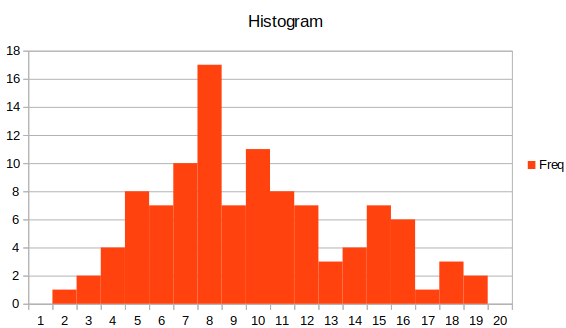
\includegraphics[scale=.60]{hist.png}
\end{center}
We also compute the $\bar{X}$ and $\bar{R}$ charts,
\begin{center}
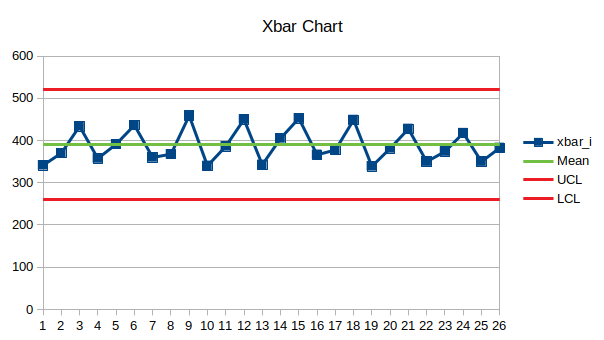
\includegraphics[scale=.75]{xbar.png}
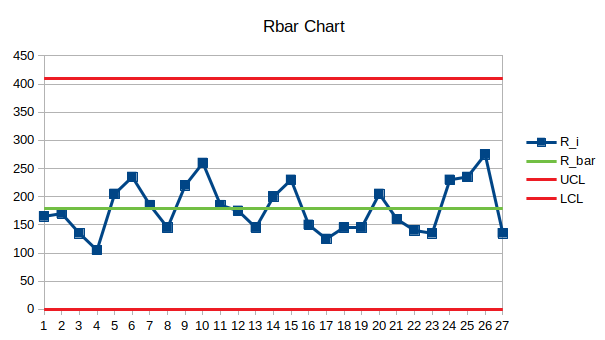
\includegraphics[scale=.75]{rbar.png}
\end{center}
We see that the process is well within control. Because of this, we continue our calculations. Now, we compute as before,
\begin{align*}
\hat{\sigma} &= \frac{\bar{R}}{d_2}\\
&=\frac{179.2592593}{2.059}\\
&=87.06132067\\
\hat{C}_p&=\frac{USL-LSL}{6\hat{\sigma}}\\
&=\frac{500-300}{6*87.06132067}\\
&=0.3831417625\\
&\to 0.38
\end{align*}
Next, we consider $\hat{C}_{pk}$. To compute, we consider the following calculations,
\begin{align*}
\zeta(USL) &= |500-390.0925926|\\
&= 109.9074074\\
\zeta(LSL) &= |390.0925926-300|\\
&=90.09259259
\end{align*}
Because we see that the second of these calculations is the smallest, we shall use it in the calculation of our $\hat{C}_{pk}$ value as,
\begin{align*}
\hat{C}_{pk} &= \frac{\bar{\bar{x}}-LSL}{3\hat{\sigma}}\\
&=\frac{390.0925926-300}{3(87.06132067)}\\
&=\frac{90.0925926}{261.183962}\\
&=0.3449392218\\
&\to 0.35
\end{align*}
Finally, we compute the DPMO as,
\begin{align*}
P(X<LSL) &=\Phi(\frac{300-390.0925926}{\hat{\sigma}})\\
&=0.150377036\\
P(X>USL) &= 1-\Phi(\frac{500-390.0925926}{\hat{\sigma}}\\
&=0.103399974\\
P(Defect) &= 0.150377036+0.103399974\\
&=0.25377701\\
DPMO &= P(Defect)\times 10^6\\
&=253777.0096\\
&\to 253777.0
\end{align*}
\end{enumerate}
\end{document}
